\heading{1. Does the end-to-end router plateau?}
\textbf{What changed?} The TinyCNN still chooses one of 213 classifiers for the entire batch. We now keep the most frequently selected classifiers resident on the GPU, ranked using only the 2,000 calibration images for each batch size. The resident count is limited by available memory, not a fixed cap. An uncached choice can still run on demand. All qualifying passes reproduced the original predictions exactly.

\def\RoutedResnetRows{%
8 & 85.05\% & 6.74 & 0.842 & 63.21 & 85.85\% & 6.86 & 0.858 & 65.84\\%
16 & 84.92\% & 8.79 & 0.549 & 40.86 & 85.85\% & 9.24 & 0.578 & 43.40\\%
32 & 84.96\% & 13.55 & 0.424 & 30.57 & 85.85\% & 14.33 & 0.449 & 32.81\\%
64 & 84.02\% & 21.21 & 0.333 & 24.25 & 85.85\% & 26.88 & 0.422 & 30.69\\%
128 & 84.02\% & 38.48 & 0.304 & 22.12 & 85.85\% & 52.14 & 0.412 & 30.46\\%
}

\begin{center}\small
\begin{tabular}{@{}rrrrrrrrr@{}}\toprule
 & \multicolumn{4}{c}{Batch router} & \multicolumn{4}{c}{Fixed ResNet101 FP16}\\
\cmidrule(lr){2-5}\cmidrule(lr){6-9}
Batch & Test acc. & ms/batch & ms/image & mJ/image & Test acc. & ms/batch & ms/image & mJ/image\\
\midrule
\RoutedResnetRows
\bottomrule\end{tabular}
\end{center}
\smallcap{Medians of qualifying passes over 10,000 CIFAR-100 test images; energy is GPU-only. At batches 8/16/32/64/128 the repeat counts were 1/3/3/2/3 for the router and 1/1/2/2/2 for ResNet101. Each pass warmed up for at least 30 seconds and 50 batches, then cooled to at most 65 degrees Celsius before timing without clearing the classifier cache. Both qualifying batch-8 passes used a 64-degree gate.}

\begin{center}\vspace{-2pt}
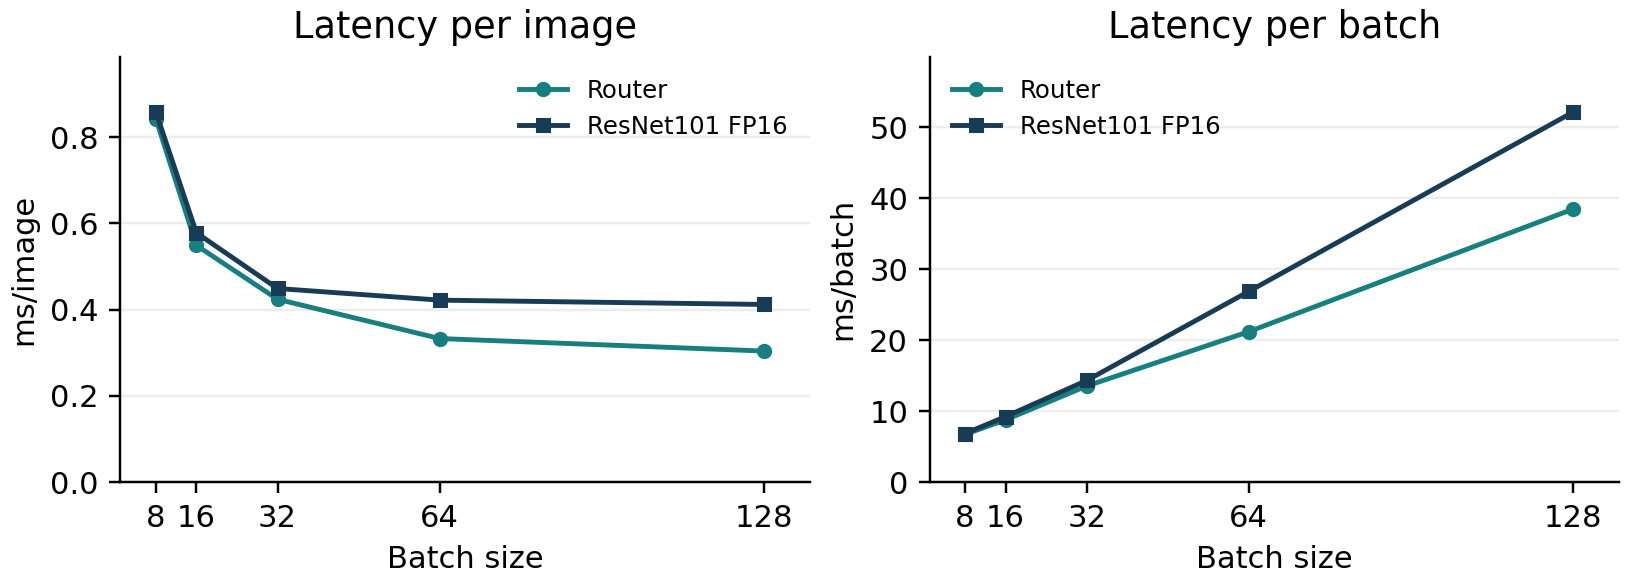
\includegraphics[width=.93\linewidth]{router-resnet101-latency.png}\\[-2pt]
\end{center}\vspace{-4pt}
\smallcap{Only qualifying table values are plotted. Time per batch includes the shorter final batch when present.}

\textbf{Did residency reduce reloads?} Calibration chose four distinct models at batch 8, three at 16, and two at each of 32, 64, and 128. All fit while leaving at least 1 GiB free. Qualifying passes had no timed disk reads. Batch 32 loaded one extra classifier from RAM per pass; batches 16, 64, and 128 needed no timed GPU loads.

\textbf{What is the trade-off?} The router was faster per image than fixed ResNet101 at every tested batch size in these measurements, but less accurate. At batch 8 the latency difference was only 0.016 ms per image, with one qualifying repeat for each path, so it is not a reliable speedup estimate. The routed batch-64 and batch-128 scores both equal 84.02\%, but the predictions differed: each got 8,402 images right, not necessarily the same images.
